% \addcontentsline{toc}{chapter}{Chapitre 1} 
\chapter{Contexte général du projet}
Ce premier chapitre a pour objectif de présenter l'organisme d'accueil, son historique, ses objectifs et ses activités. Il fournira également une description du contexte du projet, en mettant en évidence le problème qu'il vise à résoudre, les attentes associées, ainsi que la gestion et la planification de sa mise en œuvre.

\clearpage

\section{Introduction}
Cette étape consiste à faire présenter le cadre général du projet, nous commencerons par décrire l’organisme d’accueil ensuite nous présenterons le cadre et le contexte du projet pour enfin expliquer la problématique et les objectifs du projet. 


\section{Présentation de l’organisme d’accueil}
\label{sec:hotspot}
\subsection{Le groupe Société générale}
Le groupe "Société Générale" est l'un des principaux groupes de services financiers en Europe. Fondé en 1864, il reste l'une des principales banques françaises, bénéficiant d'un positionnement géographique unique entre l'Europe et l'Afrique, ainsi que des plus grands centres financiers internationaux. Grâce à un modèle axé sur la diversité, l'intégrité, la solidité financière, l'innovation et la stratégie de croissance durable, la "Société Générale" s'engage dans des transformations positives sur les plans social et économique, visant toujours à être le partenaire de confiance de ses clients. 

\medskip

Avec plus de 150 ans d'expérience en tant qu'acteur économique, et une solide présence en Europe connectée au reste du monde, le groupe compte plus de 147 000 collaborateurs dans 67 pays. Il accompagne quotidiennement 31 millions de clients particuliers, entreprises et investisseurs institutionnels, en leur proposant une large gamme de conseils et de solutions financières adaptées. Le groupe repose sur trois pôles métiers complémentaires :

\begin{itemize}

    \item[•] La banque de détail en France, représentée par les enseignes Société Générale, Crédit du Nord et Boursorama, qui offrent des services financiers complets grâce à une plateforme omnicanale à la pointe de l'innovation digitale.
    
    \item[•] La banque de détail à l'international, les services financiers et les assurances, avec des réseaux présents dans les zones géographiques en développement et des métiers spécialisés leaders sur leurs marchés respectifs.
    
    \item[•] La banque de financement et d'investissement, la banque privée, la gestion d'actifs et les métiers titres, qui se distinguent par leurs expertises reconnues, leurs positions internationales clés et leurs solutions intégrées.
    
 \end{itemize}

Le groupe "Société Générale" se distingue également par sa présence sur le marché africain, notamment au Maroc, à travers la Société Générale Maroc (SGMA) et la Société Générale African Business Services (SG ABS), cette dernière étant responsable de la direction de l'Organisation des Systèmes d'Information (DOSI).\cite{SG}

\begin{figure}[!h]
    \centering %
        
\includegraphics[height=3.5cm]{images/logos/Societe Generale.png}
    \caption{Logo de la SG}
\end{figure}

\subsection{Société générale African Business Services}
Avec une présence historique en Afrique, le Groupe Société Générale, un acteur de référence sur le marché bancaire, bénéficie d'un positionnement unique dans la région. Cela lui permet d'offrir à ses clients l'expertise et le savoir-faire d'une banque internationale, combinés à la proximité d'une banque locale. Société Générale accompagne les économies locales et compte 3,7 millions de clients, dont 150 000 entreprises.\\

Le groupe se fixe comme défi d'améliorer sa part de marché sur le continent africain en restant constamment innovant et en capitalisant sur toutes les expertises du Groupe pour renforcer sa position. Afin de consolider ce positionnement, le Groupe a renforcé son expertise technique dans la région africaine en créant un hub technologique panafricain appelé Société Générale African Business Services (SG ABS). Ce centre d'expertise se positionne comme un acteur clé dans le domaine des technologies de l'information (IT) et prévoit d'augmenter ses effectifs au cours des prochaines années, en se concentrant sur l'accompagnement des métiers dans leur stratégie de création de valeur pour leurs clients bancaires finaux. Ces besoins évoluent rapidement dans un contexte d'innovations technologiques.\\

La création de ce hub technologique s'inscrit dans la stratégie de développement du Groupe en Afrique. SG ABS bénéficiera également de la proximité avec certains partenaires technologiques importants de la banque, implantés au Maroc.\\

\begin{figure}[!h]
    \centering %
        
\includegraphics[height=1.5cm]{images/logos/SG_ABS.png}
    \caption{Logo de la SG ABS}
\end{figure}

\subsection{Fiche signalétique}
\begin{figure}[htbp]
    \centering
    \begin{longtable}{ |p{5cm}|p{7cm}| } 
        \hline
        \textcolor{gray}{Dénomination sociale} & Société Générale - African Business Services \\
        \hline
        \textcolor{gray}{Année de création} & 2018 \\
        \hline
        \textcolor{gray}{Secteur} & Banque et Finance, Centre d’expertise IT, Hub technologique panafricain, ITBancaire \\
        \hline
        \textcolor{gray}{Type} & Société anonyme, SA \\
        \hline
        \textcolor{gray}{Taille de l’entreprise} & 500 – 600 employés \\
        \hline
        \textcolor{gray}{Spécialisations} & • Centre d’expertise IT \\
        & • Hub technologique panafricain \\
        & • Banque \& Finance \\
        & • IT Bancaire \\
        & • Digital Factory \\
        & • Testing Factory \\
        & • Etudes \& Développement \\
        & • Architecture d’entreprise \\
        & • Organisation \& Processus \\
        & • Qualité \& Méthodes \\
        & • Ingénierie \& Technologies \\
        \hline
        \textcolor{gray}{Siège social} & Casablanca, Maroc \\
        \hline
        \textcolor{gray}{Adresse principale} & SOCIETE GENERALE AFRICAN BUSINESS SERVICES, Boulevard Sidi Mohamed Ben Abdellah, Tour Ivoire 2, Marina Casablanca \\
        \hline
        \textcolor{gray}{Site Web} & \url{https://particuliers.societegenerale.fr} \\
        \hline
    \end{longtable}
    \caption{Fiche signalétique de SG ABS}
    \label{fig:table}
\end{figure}

\newpage

\subsection{Organigramme de la Société générale ABS}
SG ABS est une entité globale, autonome dans ses activités, ayant pour vision de servir l’Afrique depuis l’Afrique. Il s'agit d'un centre d'expertise en technologies de l'information (IT) et d'un hub technologique panafricain, organisé autour de quatre principaux pôles :

\begin{itemize}
    \item[•] \textbf{Études \& Solutions - Métiers de la maîtrise d'ouvrage (MOA)} : Ce pôle se concentre sur les études, les solutions et les métiers liés à la gestion des projets et des besoins des clients.
    \item[•] \textbf{Infrastructure \& Production} : Ce pôle est responsable de l'infrastructure technologique et de la production des services IT, garantissant leur disponibilité et leur fonctionnement optimal.
    \item[•] \textbf{Architecture, Méthodes \& Process} : Ce pôle se focalise sur l'architecture des systèmes, les méthodologies de travail et les processus, afin d'assurer une harmonisation et une efficacité globale au sein de l'organisation.
    \item[•] \textbf{Digital Factory} : Ce pôle est dédié à l'innovation et à la transformation numérique, en développant des solutions technologiques avancées pour répondre aux besoins évolutifs des clients et aux tendances du marché.
\end{itemize}

Ces quatre pôles travaillent de manière coordonnée pour soutenir les activités de SG ABS et offrir des services de qualité à travers l'Afrique.

\begin{figure}[!h]
    \centering
        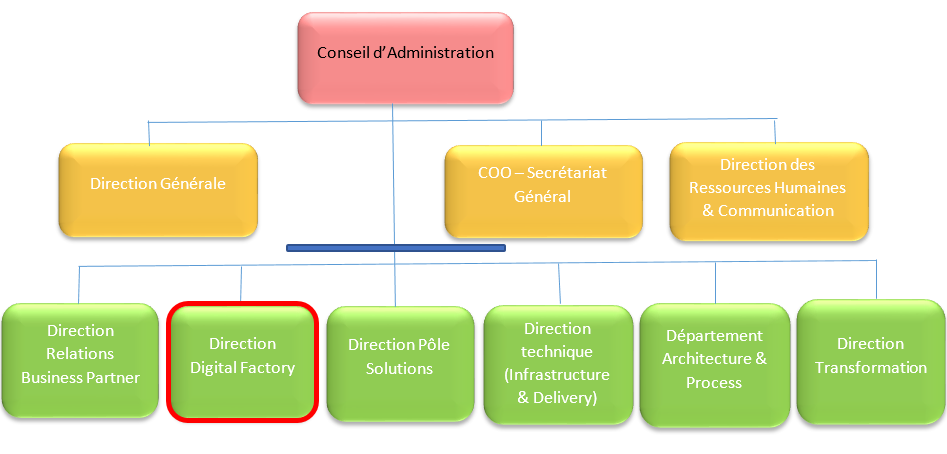
\includegraphics[width=15cm]{images/contexte/ogranigramme2.png}
        \caption{Organigramme de la SG ABS}
\end{figure}
\medskip

\newpage

\subsection{Présentation de la Digital Factory}
\textbf{\large{La raison d'être et les objectifs de la Digital Factory SGABS}}

\medskip
Face aux opportunités stratégiques offertes par le numérique pour le groupe Société Générale, l'entité "Digital Factory" a été créée. Cette entité est chargée de conduire la transformation digitale du groupe et de renforcer la culture numérique.\\

La Digital Factory est un lieu collaboratif et innovant, qui a récemment émergé dans plusieurs entreprises en Europe et aux États-Unis. Il s'agit d'un laboratoire dédié à l'innovation, rassemblant des équipes aux profils pluridisciplinaires engagées dans la transformation globale de l'entreprise.\\

Dans le cadre de cette transformation digitale, la Digital Factory vise à développer des solutions digitales pour les filiales de la région AFS, en travaillant en étroite collaboration avec le Hub Marketing des directions régionales AFS. L'objectif est de répondre rapidement à la concurrence croissante en Afrique. La Digital Factory SGABS devient ainsi un accélérateur de la transformation digitale pour les filiales AFS et a mis en place :

\begin{itemize}
    \item[•] Un Product Management Agile, pour construire de manière itérative et progressive des produits basés sur la valeur.
    \item[•] Une approche centrée sur le client (UX Design), visant à accroître la satisfaction client en termes de qualité et de délai.
    \item[•] L'industrialisation des processus de livraison des mises à jour (CI/CD), afin de réduire le Time To Market.
    \item[•] La mise en place de provisionnement automatique des environnements, permettant une meilleure maîtrise du retour sur investissement (ROI) des infrastructures de nos solutions digitales.
    \item[•] La garantie d'une interopérabilité fonctionnelle et technologique grâce à une plateforme digitale évolutive et innovante.
    \item[•] La création d'usines logicielles pour fiabiliser la conception et la réalisation des solutions digitales.
    \item[•] Toutes ces initiatives contribuent à servir le continent africain depuis l'Afrique, en partageant des sensibilités et des cultures communes.\\
\end{itemize}

\textbf{\large{Types de projets}}
\medskip
\begin{itemize}
    \item[•] Solutions innovantes multicanales (web, mobile, digital corner) au bénéfice des clients ou des collaborateurs.
    \item[•] Projets qui ne nécessitent pas une évolution du CBS (Core Banking System) (hors interfaces - SMG/API).
    \item[•] Développements internes.\\
\end{itemize}

\textbf{\large{Organisation}}

\medskip
La Digital Factory est organisée en quatre équipes pluridisciplinaires, fonctionnant en mode Agile et en interaction avec les fonctions supports centrales (Architecture, GTS, Compliance, Marketing, Architecture, etc.) et les filiales.\\

L'organisation des équipes de la Digital Factory est présentée dans la figure suivante :

\begin{figure}[!h]
    \centering
        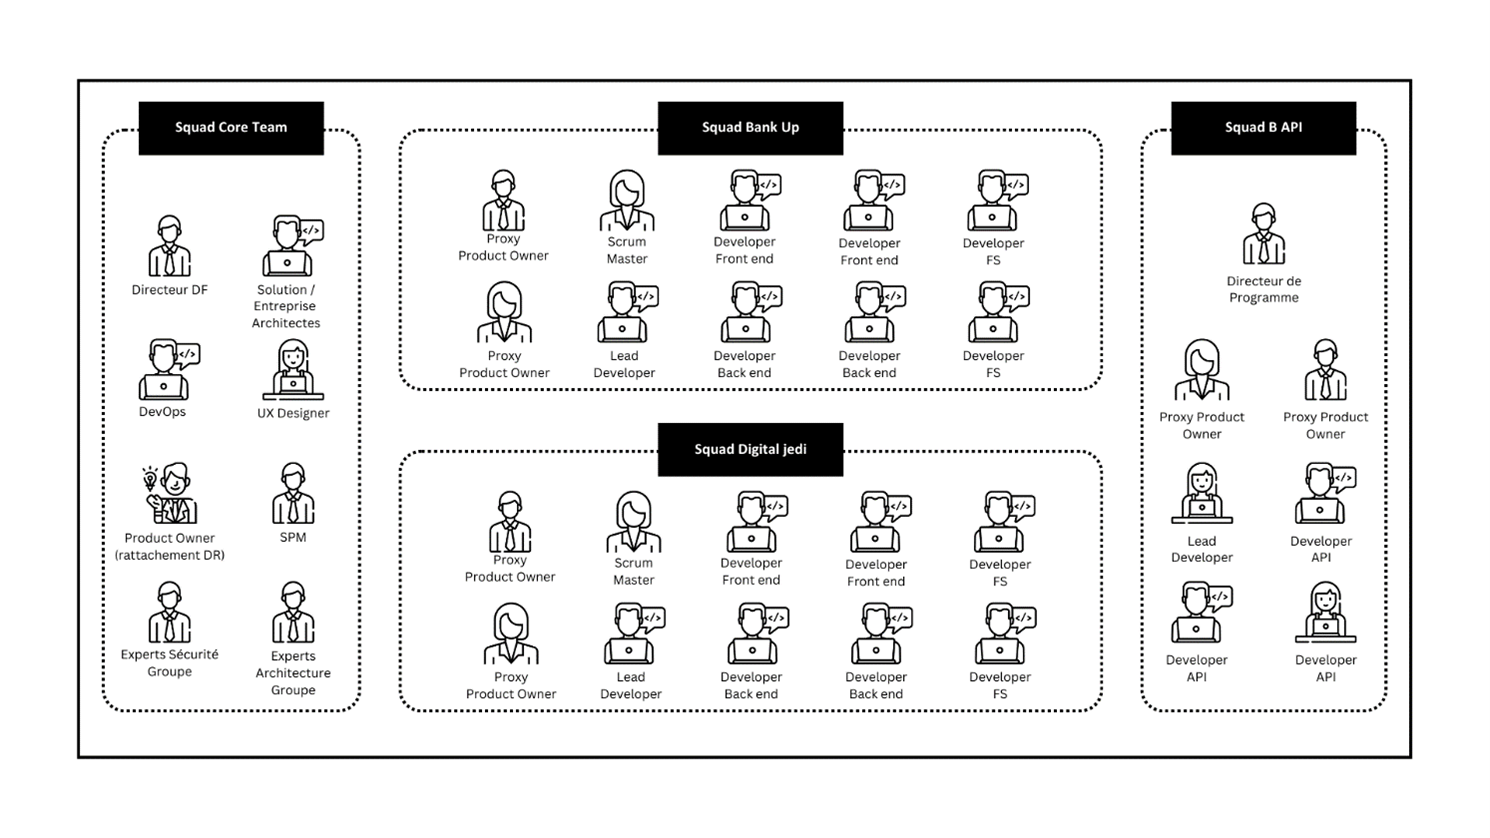
\includegraphics[width=15cm]{images/contexte/Difa.png}
        \caption{Organigramme de la Digital Factory}
\end{figure}

\begin{itemize}
    \item[•] \textbf{Core Team} : Cette équipe est composée d'un Directeur de la Digital Factory, de Solution Architectes, DevOps, UX Designer, Product Owner, SPM, Experts Sécurité Groupe et Experts Architecture Groupe. Cette équipe interagit avec tous les projets des autres équipes de la Digital Factory.
    \item[•] \textbf{Digital JEDI / OPEN R} : Cette équipe s'inscrit dans la stratégie de digitalisation de la banque, visant à rattraper la concurrence et à orienter le flux actuel de clients Retail de l'agence vers la zone digitale. Elle se focalise sur l'industrialisation des deux processus développés au Ghana : "Open App" (application) destinée à l'ouverture de comptes Retail en agences et hors agences (entreprises, universités, etc.) et "Digit" (application bancaire Digital Corner accessible 24/7 sur des zones digitales, dotée des fonctionnalités nécessaires pour couvrir les besoins quotidiens des clients).
    \item[•] \textbf{B-API / UNIBANK} : Cette équipe permet de connecter rapidement les applications (hébergées en interne ou externe) aux CBS des différentes filiales de la zone AFS. Elle assure un accès unifié et sécurisé (authentification de l'utilisateur basée sur des standards, gestion des habilitations et piste d'audit) en faisant abstraction des SMGs sous forme d'APIs (Application Programming Interface). B-API est une composante technique structurante de la plateforme Digital Banking construite avec le projet Bank-UP.
    \item[•] \textbf{Bank-UP} : Cette équipe a pour objectif la mise en place d'une plateforme digitale mutualisée au service des filiales de la Zone AFS. Il s'agit d'une application bancaire en ligne (web et mobile) conforme aux attentes du Groupe en termes de time to market, sécurité, risques opérationnels et solution In-house avec propriété du code source et garantie d'évolutivité de la plateforme.\\
\end{itemize}

\section{Présentation du contexte du projet }
\subsection{Contexte du projet}
La transformation numérique est devenue un enjeu économique et sociétal majeur, remettant en question les modèles économiques, les processus de travail et les relations professionnelles. Dans ce contexte de disruption technologique et de complexité croissante des écosystèmes économiques, la SGABS a pris l'initiative de se transformer pour rester compétitive. Pour cela, elle a établi une vision stratégique claire, basée sur des plans d'action transparents et partagés en interne.\\

La mise en place de la plateforme digitale SG CONNECT fait partie intégrante de cette vision stratégique. Cette plateforme est composée de bibliothèques front-end (web, mobile) contenant les parcours clients, ainsi que d'une couche d'API permettant de masquer la complexité technique vis-à-vis des applications communiquant avec le système d'information de la SGABS. Cette approche d'Open Banking favorise l'ouverture du système d'information de la SGABS et facilite le partage sécurisé des données avec des tiers, dans le respect du consentement des clients.\\

Ce projet s'inscrit dans une démarche plus large de digitalisation de gestion optimale des produits bancaires et de l'expérience client, en leur offrant une expérience bancaire numérique moderne, personnalisée et sécurisée. Il s'appuie sur le moteur Back-End du projet UNIBANK, qui fait partie de la roadmap des projets planifiés par la Digital Factory de la SGABS.

\subsection{Problématique}
Dans un monde de plus en plus numérique et connecté, l'accès facile et pratique aux informations financières est devenu une attente primordiale des clients bancaires. Le projet d'ajout de nouvelles fonctionnalités dans l'application SG CONNECT, développé par l'équipe Bank UP, vise à répondre à cette demande en offrant aux clients de la Société Générale des fonctionnalités avancées liées à leurs cartes monétiques, transactions et produits souscrits.\\

Actuellement, les clients rencontrent plusieurs problématiques lorsqu'ils souhaitent consulter les informations relatives à leurs cartes monétiques. Ils manquent d'une vue d'ensemble claire de leurs cartes et des transactions qui y sont associées. De plus, la connaissance des plafonds nationaux et internationaux associés à chaque carte peut être limitée, ce qui peut entraîner des difficultés lors de voyages ou de transactions spécifiques.\\

De même, l'accès aux détails de leurs produits souscrits représente un défi pour les clients. Ils peuvent se retrouver dans une situation où ils ne sont pas en mesure de visualiser facilement les produits qu'ils ont souscrits, tels que des comptes spécifiques, des prêts ou des services financiers complémentaires. Cela entraîne une confusion et un manque de transparence dans la gestion de leurs finances.\\

Le projet vise donc à résoudre ces problématiques en ajoutant de nouvelles fonctionnalités dans l'application SG CONNECT. Les clients pourront désormais accéder à une vue claire de leurs cartes monétiques, avec la possibilité de consulter les transactions associées à chacune d'entre elles. De plus, ils auront la possibilité de visualiser et de gérer les plafonds nationaux et internationaux de leurs cartes, offrant ainsi un meilleur contrôle de leurs transactions.\\

En ce qui concerne les produits souscrits, les clients pourront consulter facilement les détails et les caractéristiques de leurs comptes, prêts et autres services financiers. Cette fonctionnalité offrira une visibilité accrue sur les engagements financiers des clients, ainsi qu'une meilleure compréhension des conditions et des avantages associés à chaque produit.\\

En résolvant ces problématiques, le projet vise à améliorer l'expérience client en offrant un accès pratique, transparent et autonome aux informations financières. Les clients pourront ainsi gérer leurs finances de manière plus efficace et prendre des décisions éclairées en fonction de leurs besoins et de leurs objectifs.

\subsection{Besoins et objectifs}
Le projet d'ajout de nouvelles fonctionnalités dans l'application SG CONNECT, mené par l'équipe Bank UP, a été initié pour répondre aux besoins et objectifs suivants :

\begin{itemize}
    \item[•] \textbf{Améliorer l'accessibilité aux informations financières} : Les clients de la Société Générale recherchent une plateforme conviviale et pratique pour accéder à leurs données financières. Ils souhaitent consulter facilement les détails de leurs cartes monétiques, les transactions effectuées et les plafonds associés. De plus, ils ont besoin d'un moyen simple et rapide pour visualiser les produits qu'ils ont souscrits, tels que les comptes, les prêts et autres services financiers.
    \item[•] \textbf{Renforcer la transparence et la gestion des finances personnelles} : Les clients souhaitent avoir une vue claire et complète de leurs finances. Ils ont besoin de comprendre les mouvements sur leurs cartes, les transactions effectuées, ainsi que les plafonds de dépenses autorisés. De plus, ils cherchent à avoir une vision globale de leurs produits souscrits, avec une compréhension claire des conditions, des avantages et des échéances associés.
    \item[•] \textbf{Offrir une meilleure autonomie et flexibilité} : Les clients souhaitent être en mesure de gérer leurs finances de manière autonome, sans dépendre systématiquement de l'assistance d'un conseiller en agence. Ils veulent pouvoir ajuster les plafonds de leurs cartes selon leurs besoins, consulter rapidement leurs transactions passées et actuelles, et obtenir des informations précises sur leurs produits financiers, sans contraintes de temps ni de lieu.
    \item[•] \textbf{Renforcer la confiance et la fidélité des clients} : En offrant des fonctionnalités avancées et une expérience utilisateur améliorée, le projet vise à renforcer la confiance des clients envers la Société Générale. Les clients bénéficieront d'un accès sécurisé à leurs données financières, d'une transparence accrue dans la gestion de leurs comptes et de la possibilité de prendre des décisions éclairées en matière de finances personnelles. Cela contribuera à renforcer la satisfaction et la fidélité des clients envers la banque.
\end{itemize}
En répondant à ces besoins et objectifs, le projet d'ajout de nouvelles fonctionnalités dans l'application SG CONNECT vise à offrir une expérience client optimisée, en mettant à disposition des outils et des informations essentiels pour la gestion de leurs finances personnelles. En mettant l'accent sur l'accessibilité, la transparence et l'autonomie, l'équipe Bank UP aspire à fournir une solution complète qui répond aux attentes des clients et les accompagne dans leur parcours financier.

\section{Conduite du projet}
\subsection{Méthodologie de travail : SCRUM}
La conduite de ce projet s'appuie sur la méthodologie SCRUM, adoptée par l'équipe de la Digital Factory pour garantir des résultats rapides et un time to market réduit. SCRUM est une approche agile qui permet une meilleure organisation des différentes phases du projet, en accordant une importance primordiale à l'implication et à la participation active du client tout au long du processus de développement. En suivant SCRUM, nous visons à améliorer la productivité de notre équipe, à respecter les délais fixés et à assurer le bon déroulement général du projet.

\begin{figure}[!h]
    \centering %
        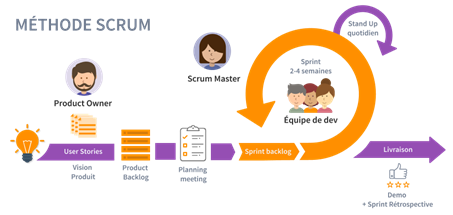
\includegraphics[width=14cm]{images/conduite/SCRUM.png}
    \caption{Méthode SCRUM}
\end{figure}

\textbf{\large{Les avantages de la méthode SCRUM}}
\medskip
\begin{itemize}
    \item[•] \textbf{Personnel engagé :} SCRUM favorise l'engagement du personnel en les impliquant activement dans la définition des activités et des horaires, ce qui conduit à une plus grande motivation et implication.
    \item[•] \textbf{Meilleure vue d’ensemble du projet :} SCRUM permet à tous les membres de l'équipe d'avoir une compréhension homogène des objectifs et des tâches à accomplir, offrant ainsi une meilleure vue d'ensemble du projet.
    \item[•] \textbf{Mise à jour des priorités :} Avec SCRUM, le client bénéficie d'une flexibilité au niveau de la définition et de l'évolution des priorités et des séquences d'activités, permettant une adaptation aux besoins changeants.
    \item[•] \textbf{Qualité du produit mise en avant :} SCRUM se concentre davantage sur la fourniture d'un service de valeur au client plutôt que sur une date limite stricte, mettant ainsi en avant la qualité du produit.
    \item[•] \textbf{Communication renforcée :} SCRUM favorise une communication régulière et transparente au sein de l'équipe, permettant une collaboration efficace et une résolution rapide des problèmes.
    \item[•] \textbf{Réduction des risques :} En utilisant des itérations courtes et des revues régulières, SCRUM permet de détecter et de résoudre les problèmes plus rapidement, réduisant ainsi les risques liés au projet.\\
\end{itemize}


\textbf{\large{Répartition des rôles dans SCRUM}}
\medskip
\begin{itemize}
    \item[•] \textbf{Le Scrum Master :} Il est responsable de la compréhension, de l'adhésion et de la mise en œuvre de la méthode SCRUM. Le Scrum Master facilite la communication au sein de l'équipe et cherche à maximiser sa productivité. Il veille également au respect des principes et des valeurs de SCRUM.
    \item[•] \textbf{Le Product Owner :} Il porte la vision du produit à réaliser et travaille en interaction avec l'équipe de développement. Le Product Owner établit les priorités des fonctionnalités à développer ou à corriger et valide les fonctionnalités terminées. Il est responsable de la gestion du product backlog et s'assure que les besoins du client sont correctement pris en compte.
    \item[•] \textbf{L'équipe de développement :} Elle est chargée de transformer les besoins définis par le Product Owner en fonctionnalités utilisables. Les décisions au sein de l'équipe de développement sont prises collectivement, sans notion de hiérarchie.\\
\end{itemize}


\textbf{\large{Les différents événements de la SCRUM}}
\medskip
\begin{itemize}
    \item[•] \textbf{Le sprint :} Il s'agit d'une itération de quelques semaines pendant laquelle une version terminée et utilisable du produit est réalisée. Un nouveau sprint commence immédiatement après la fin du précédent. Chaque sprint a un objectif clair et une liste de fonctionnalités à réaliser.
    \item[•] \textbf{La planification d'un sprint :} C'est une réunion qui précède le début d'un sprint et qui vise à définir les tâches à accomplir pendant cette période. L'équipe de développement et le Product Owner collaborent pour déterminer les objectifs et les priorités du sprint.
    \item[•] \textbf{La revue de sprint :} À la fin de chaque sprint, une réunion de revue est organisée pour présenter les fonctionnalités réalisées à l'équipe de développement et aux parties prenantes. C'est l'occasion de valider ce qui a été accompli et de recueillir des feedbacks.
    \item[•] \textbf{La rétrospective de sprint :} Elle se tient après la revue de sprint et permet à l'équipe de passer en revue le sprint écoulé afin d'identifier les aspects positifs, les problèmes rencontrés et les opportunités d'amélioration. Cela permet d'ajuster les pratiques et d'optimiser la performance pour les sprints suivants.
    \item[•] \textbf{Le daily scrum :} C'est une réunion quotidienne de courte durée au cours de laquelle l'équipe de développement fait le point sur sa progression. Les membres de l'équipe répondent à trois questions clés : qu'ont-ils réalisé la veille, qu'accompliront-ils aujourd'hui et quels sont les obstacles éventuels.\\
\end{itemize}

\textbf{\large{Les artefacts de SCRUM}}
\medskip
\begin{itemize}
    \item[•] \textbf{Le product backlog :} Il s'agit d'une liste hiérarchisée des exigences initiales du client concernant le produit à réaliser. Ce document évolue tout au long du projet en fonction des besoins du client, et le Product Owner en est responsable.
    \item[•] \textbf{Le sprint backlog :} Il représente le plan détaillé de la réalisation des objectifs d'un sprint, regroupant l'ensemble des user stories que l'équipe s'est engagée à accomplir. Il est défini lors de la réunion de planification du sprint et est régulièrement mis à jour pour suivre la progression.
    \item[•] \textbf{L'incrément :} Il correspond à la somme des éléments terminés du product backlog au cours d'un sprint, ainsi que des incréments des sprints précédents. À la fin d'un sprint, l'incrément doit être "Done", c'est-à-dire utilisable et conforme à la définition de "Done" définie par l'équipe SCRUM. Le Product Owner décide de sa libération ou non.
\end{itemize}

\subsection{Cycle de vie du projet}

\par Afin d’assurer le bon déroulement du projet, nous avons opté pour le cycle de vie suivant :
\begin{itemize}
    \item[$\bullet$] \textbf{Etude de cadrage:} cette étape consiste à bien définir le périmètre fonctionnel du projet. Elle permet de comprendre et analyser la structure de l’existant pour bien cadrer les besoins du client afin d’aboutir à un résultat qui s’aligne parfaitement avec ses attentes.
    \item[$\bullet$] \textbf{Spécifications et analyse des besoins:} cette phase permet de spécifier les besoins
définis dans la précédente phase du projet. Elle est d’une grande signification, 
    \item[$\bullet$] \textbf{Développement:} C'est la partie où l'on développe les fonctionnalités et les besoins exprimés lors de la phase précédente. L'objectif est de produire des services conformes aux spécifications exprimées par le métier tout en respectant un ensemble de règles de gestion technique et de bonnes pratiques.
    \item[$\bullet$] \textbf{Tests et validation:} Ils sont réalisés à la fin de chaque Sprint pour valider le travail réalisé avec le client.
    \item[$\bullet$] \textbf{Déploiement:} C'est la partie où les services développés et testés sont déployés dans un environnement accessible au client pour qu'il puisse les utiliser.
    \item[$\bullet$] \textbf{Monitoring:} À ce niveau, nous gardons un œil sur l'application en cours d'exécution et sommes prêts pour résoudre tout problème lorsqu'il se produit. 
\end{itemize}


\subsection{Planification du projet}
Pour gérer le projet et aboutir aux objectifs fixés ci-dessus, nous avons suivi les étapes représentées dans le diagramme de GANTT suivant :

\begin{figure}[!h]
    \centering %
        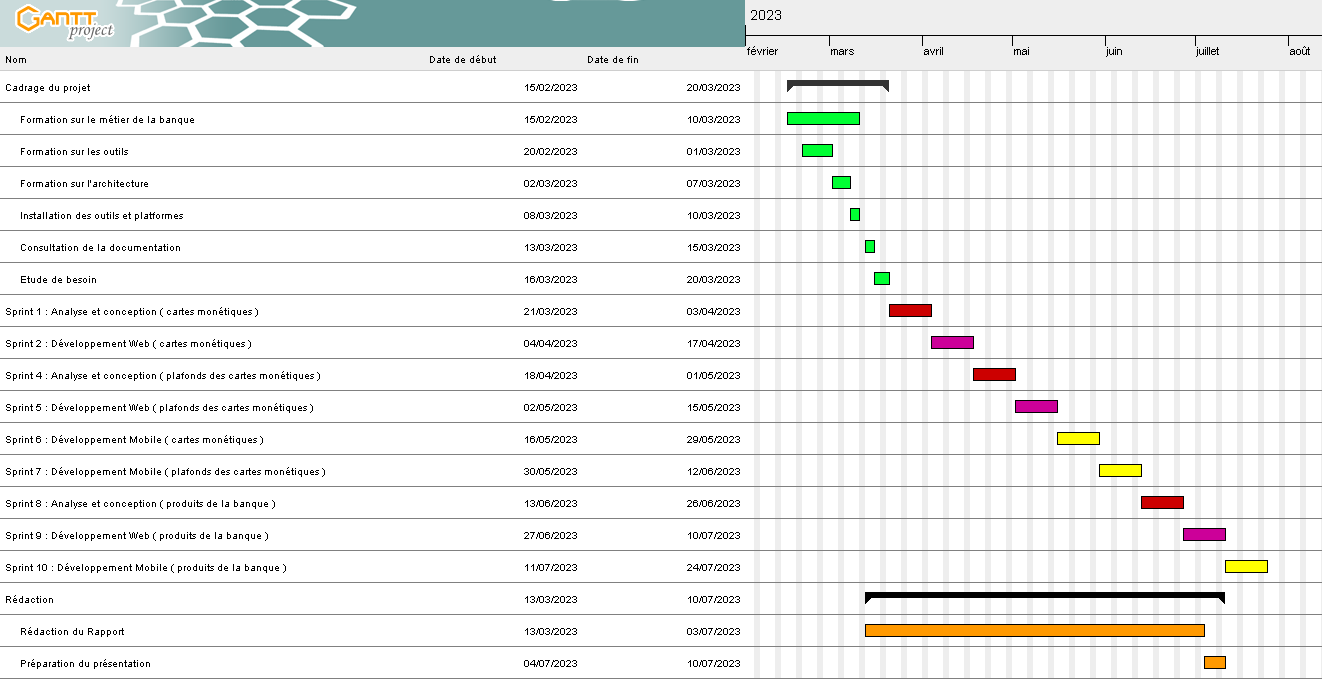
\includegraphics[width=16cm]{images/conduite/gantt.png}
    \caption{Diagramme de Gantt}
\end{figure}

\newpage

La phase de planification du projet a débuté par une étape de cadrage, au cours de laquelle nous avons bénéficié de formations approfondies afin de comprendre le domaine bancaire et de nous familiariser avec les exigences spécifiques du projet. Cette phase nous a permis de mener une étude approfondie des besoins et de spécifier les fonctionnalités à mettre en œuvre.\\

Pour mettre en pratique la méthodologie SCRUM, nous avons créé un backlog qui regroupe toutes les fonctionnalités requises sous forme de user stories. Lors de la réunion de planification du sprint, appelée "sprint planning", nous avons sélectionné les user stories sur lesquelles nous allons travailler pour chaque sprint. Ensuite, nous avons procédé à l'analyse et à la conception de chaque fonctionnalité, avant de passer à sa mise en œuvre.\\

Le développement de chaque fonctionnalité s'est déroulé au sein de sprints définis, où elle a été développée, testée, corrigée et déployée. À la fin de chaque sprint, nous avons obtenu une version fonctionnelle du produit, prête à être évaluée et validée par l'équipe de développement et les parties prenantes.\\

Cette approche itérative nous a permis de travailler de manière efficace et d'assurer une progression continue du projet, tout en offrant une flexibilité pour s'adapter aux éventuels changements de priorités ou de besoins.


\subsection{Outils de gestion de projet}

Pour mener à bien le projet, l'utilisation d'outils de gestion est essentielle afin de faciliter le travail d'équipe et de garantir le respect de la méthodologie Scrum. Trois outils ont été employés dans ce contexte : Jira, Microsoft Teams et Confluence.

\begin{itemize}
\item[$\bullet$] \textbf{Jira}
\end{itemize}
Jira a été utilisé comme outil de gestion de projet en ligne par la Société Générale African Business Services. Il s'agit d'une plateforme polyvalente qui facilite la gestion de projet en permettant le suivi des tâches, l'identification des obstacles et le partage d'informations au sein de l'équipe. Jira est basé sur l'organisation des projets en tickets, chacun représentant une tâche spécifique. Il offre également la possibilité de suivre l'état des tickets et de définir un flux de travail adapté aux méthodes de travail.\\
Jira génère des graphiques et des visualisations qui permettent de visualiser rapidement l'état des différentes missions et d'identifier les problèmes à résoudre en priorité.\\
Dans notre projet, Jira a été utilisé pour publier les User Stories, organiser les sprints et le backlog, suivre les tâches et sous-tâches, ainsi que pour estimer l'effort de l'équipe.
\begin{figure}[!h]
    \centering %
        
\includegraphics[height=3cm]{images/logos/jira.png}
    \caption{Logo de Jira}
\end{figure}

\begin{itemize}
    \item[$\bullet$] \textbf{Microsoft Teams}
    \end{itemize}
    Microsoft Teams a été utilisé pour organiser les réunions entre les membres de l'équipe. Cet outil a permis aux membres de l'équipe de communiquer, de planifier les tâches, de partager des astuces utiles, de discuter des progrès réalisés, des tâches à accomplir et des difficultés rencontrées. Des sessions de formation ont également été programmées pour renforcer la compréhension des fondements du métier bancaire dans notre domaine. Microsoft Teams a également été utilisé pour planifier les différentes cérémonies Scrum.
    \begin{figure}[!h]
        \centering %
            
\includegraphics[height=3cm]{images/logos/microsoftTeams.png}
        \caption{Logo de Microsoft Teams}
    \end{figure}

    \begin{itemize}
        \item[$\bullet$] \textbf{Confluence}
        \end{itemize}
        Confluence est une solution de travail collaboratif qui permet de créer et de stocker des fichiers sur une plateforme unique. Il offre la possibilité de créer des pages à partir de zéro ou d'utiliser des modèles personnalisables parmi une large sélection. Les pages créées peuvent être enrichies en commentaires, images, vidéos ou GIF, et peuvent être liées dans un espace dédié, permettant aux membres de l'équipe de partager leurs impressions, de demander de l'aide et de faciliter la prise de décision.
        \begin{figure}[!h]
            \centering %
                
\includegraphics[height=3cm]{images/logos/Confluence.png}
            \caption{Logo de Confluence}
        \end{figure}

Ces trois outils ont joué un rôle essentiel dans la gestion du projet en favorisant la collaboration, l'organisation et le partage d'informations au sein de l'équipe de développement.

\newpage

\section{Conclusion}
En conclusion, nous avons présenté le cadre générale du projet, l'organisme d'accueil, son historique, ses objectifs et ses activités, puis nous avons passé à la méthodologie adoptée, le cycle de vie du projet et la planification à l'aide du diagramme de Gantt. Nous avons également examiné les outils de gestion du projet utilisés pour faciliter la coordination et le suivi de l'équipe. Ces éléments sont essentiels pour assurer une gestion efficace du projet, respecter les délais et atteindre les objectifs fixés.\\
Dans le chapitre suivant, nous aborderons l'analyse des besoins, la modélisation et la conception du projet.